\documentclass[./main.tex]{subfiles}

\begin{document}
\onehalfspacing
\section{Կապակցված տարածություն, կապակցված ենթաբազմություն։ Թեո\-րեմ\-ներ կապակցված ենթաբազմությունների միավորման և կապա\-կցված ենթաբազմության փակման մասին։ Կապակցվածության բաղադ\-րիչ, ոչ հոմեոմորֆ տարածությունների օրինակներ։}\label{sec:14}

% 1 +
\par Եթե ունենք $(X, \tau)$ և $(Y, \sigma)$ տոպոլոգիական տարածություններ, ընդ որում $X \cap Y =\varnothing$, ապա $X \cup Y$ բազմությունը կարելի է վերածել տոպոլոգիական տարածության՝ համարելով $X \cup Y$-ում բաց ենթաբազմություններ նրա այն բոլոր $U$ ենթա\-բազ\-մու\-թյուն\-ները, երբ $U \cap X$ և $U \cap Y$ ենթաբազմությունները բաց են համապատաս\-խա\-նա\-բար $X$-ում և $Y$-ում։ Տոպոլոգիայի 1-3 աքսիոմները ստուգվում են հեշտությամբ։ Նկա\-տենք, որ ստացված տոպոլոգիական տարածությունում $X$ և $Y$ ենթաբազմու\-թյուն\-նե\-րը ոչ դատարկ, չհատվող, միաժամանակ բաց և փակ ենթաբազմություններ են։ Այս տարածությունը կոչվում է $X$ և $Y$ տարածությունների \textbf{չկապակցված միա\-վո\-րում}։

% 2 + 
\begin{definition}
Տոպոլոգիական տարածությունը կոչվում է \textbf{կապակցված տարա\-ծու\-թյուն}, եթե այն չի կարող ներկայացվել որպես իր երկու ոչ դատարկ, չհատվող, բաց ենթա\-բազ\-մութ\-յուն\-ների միավորման տեսքով։
% 3 +
\par Համարժեք ձևակերպում․ տարածությունը կապակցված է, եթե այն չի կարող ներկայացվել որպես իր երկու ոչ դատարկ, չհատվող փակ ենթաբազմությունների միավորման տեսքով։
% 4 +
\par Եվս մի համարժեք ձևակերպում․ $X$ տոպոլոգիական տարածությունը կապակց\-ված է, եթե $X$-ում գոյություն ունի միայն մի ոչ դատարկ, միաժամանակ բաց և փակ ենթա\-բազ\-մութ\-յուն՝ ինքը $X$-ը։
\end{definition}
% 5 +
\begin{definition}
 $X$ տոպոլոգիական տարածության $Y$ ենթաբազմությունը կոչվում է \textbf{$\boldsymbol{X}$-ի կապակցված ենթաբազմություն}, եթե $Y$-ը կապակցված տարածություն է $X$-ից նրա վրա մակածված տոպոլոգիայով։
\end{definition}
% 6 +
\begin{example}\label{ch14ex1}
\label{15:օրինակ 1}
ա) Ցանկացած անտիդիսկրետ տարածություն կապակցված տարա\-ծութ\-յուն է։ բ) Մեկից ավելի կետեր պարունակող ամեն մի դիսկրետ տարածություն կապակցված չէ։ գ) $(\R, \textrm{սովոր.})$ թվային ուղղի $(-\infty, 0)\cup(0, +\infty)$, $(0,1)\cup(1,2)$ և $\Z=\{0, \pm 1, \pm2, \dots\}$ ենթաբազմությունները կապակցված չեն (\textbf{ինչո՞ւ})։
\end{example}

% 7
\begin{theorem}\label{ch14thm1}
\label{15:թեորեմ1}
Թվային ուղղի $[a,b]$ հատվածը կապակցված տարածություն է ($\R$-ի սովորական մետրիկային տոպոլոգիայից մակածված տոպոլոգիայով)։
\end{theorem}
% 8
\begin{proof}
Դիցուք $[a,b]=U\cup V$, որտեղ $U$-ն և $V$-ն չհատվող, ոչ դատարկ, բաց (հետևաբար նաև փակ) ենթաբազմություններ են։ Որոշակիության համար ենթադրենք $a\in U$ և դիտար\-կենք $U$-ի ենթաբազմությունը կազմված $U$-ի այն բոլոր տարրերից, որոնք փոքր են $V$-ի բոլոր տարրերից՝ $W=\{u\in U\mid u < v,\, \forall v \in V \}$։ Քանի որ $a\in W$, ուստի $W \neq \varnothing$։ Նշանակենք $h$-ով $W$ ենթաբազմության ճշգրիտ վերին եզրը՝ $h=\sup W$։ Քանի որ $h$-ը հպման կետ է $W$-ի համար, և $W \subset U$, ուստի $h$-ը հպման կետ է նաև $U$-ի համար։ Հետևաբար $h\in \widebar{U} = U$, ուրեմն $h\in W$ (ինչո՞ւ)։ Մյուս կողմից՝ ցանկացած $\varepsilon > 0$ թվի համար $(h-\varepsilon,\, h+\varepsilon) \cap V \neq \varnothing$։ Հակառակ դեպքում, եթե $(h-\varepsilon_0,\, h+\varepsilon_0 ) \cap V=\varnothing$ որևէ $\varepsilon_0$-ի համար, ապա կունենանք, որ $V$-ի բոլոր տարրերը մեծ կամ հավասար են $h + \varepsilon_0$ թվից։ Իսկ դրանից կհետևի, որ օրի\-նակ $h+\dfrac{\varepsilon_0}{2}\in W$, և ուրեմն $h \neq \sup W$։

%$(h-\varepsilon_0,h+\varepsilon_0) \subset U_0\ \Rightarrow\ \left(h+\dfrac{\varepsilon_0}{2}\right) \in W\ \Rightarrow\ h \neq \sup W$):
% 9 +
\par Նշանակում է՝ $h$-ը հպման կետ է նաև $V$-ի համար, ուստի $h \in \overline{V} = V$։ Այսպիսով ստացանք $h \in U \cap V$ (հակասություն)։
\end{proof}

% 10 + 
\begin{theorem}\label{ch14thm2}
\label{15:թեորեմ 2}
Կապակցված տարածության կերպարը անընդհատ արտապատ\-կեր\-ման դեպքում կապակցված տարածություն է։
\end{theorem}
% 11 +
\begin{proof}
Դիցուք $X$-ը կապակցված է, $f:X \rightarrow Y$ անընդհատ է և $f(X)=Y$։ Ենթադրենք $Y=U \cup V$, որտեղ $U$-ն և $V$-ն ոչ դատարկ, չհատվող, բաց ենթա\-բազ\-մութ\-յուն\-ներ են $Y$-ում։ Պարզ է, որ $f^{-1}(U),\, f^{-1}(V)$-ն ոչ դատարկ, բաց ենթա\-բազ\-մութ\-յուն\-ներ են $X$-ում և $f^{-1}(U) \cup f^{-1}(V) = X,\ f^{-1}(U) \cap f^{-1}(V)= \varnothing$։ Ստացվեց, որ $X$-ը կա\-պակցված չէ (հակասություն):
\end{proof}
% 12 +
\begin{hetevanq}\label{ch14cor1}
Կապակցվածությունը տոպոլոգիական հատկություն է (\textbf{հիմնավո\-րե՛ք})։
\end{hetevanq}
% 13 +
\begin{theorem}\label{ch14thm3}
\label{15:թեորեմ 3}
Դիցուք ունենք $X$ տարածության $Y_i \subset X,\ i \in I$ կապակցված ենթա\-բազ\-մութ\-յուն\-ներ։ Եթե նրանց հատումը դատարկ չէ, ապա նրանց $Y=\bigcup\limits_i Y_i$ միա\-վո\-րումը նույնպես $X$-ի կապակցված ենթաբազմություն է։ 
\end{theorem} 

% 14 +
\begin{proof}
Դիցուք $U$-ն կամայական ոչ դատարկ, միաժամանակ բաց և փակ ենթա\-բազ\-մութ\-յուն է $Y$-ում։ Ցույց տանք, որ այն համընկնում է $Y$-ի հետ (դրանից կհետևի, որ $Y$-ը կապակցված է)։ Գոյություն ունի $i_0 \in I$, որ $U \cap Y_{i_{_0}} \neq \varnothing$։ Պարզ է, որ $U \cap Y_{i_{_0}}$-ն ոչ դատարկ, միաժամանակ բաց և փակ ենթաբազմություն է $Y_{i_{_0}}$-ում, ուստի $U \cap Y_{i_{_0}}=Y_{i_{_0}}$ (շնորհիվ $Y_{i_{_0}}$-ի կապակցվածության)։ Նշանակում է՝ $Y_{i_{_0}} \subset U$։ Կամայական $i \neq i_0$ ինդեքսի դեպքում, քանի որ $Y_{i_{_0}} \cap Y_i \neq \varnothing$, ուստի $U \cap Y_{i} \neq \varnothing$։ Այժմ, կատարելով վերը բերված դատողությունները արդեն $Y_i$ և $U$ ենթաբազմությունների համար, ստանում ենք, որ $Y_i \subset U$։ Հետևաբար $\bigcup\limits_i Y_i \subset U$, և ուրեմն $U=Y$։
\end{proof} 

\begin{hetevanq}\label{ch14cor2}
$\R$ թվային ուղիղը կապակցված է, քանի որ $\R= \bigcup\limits_{n \in \N} [-n;n]$ և ${\bigcap\limits_{n \in \N} [-n;n] \neq \varnothing}$, իսկ $[-n;n],\, n \in \N$ հատվածները կապակցված են ըստ \hyperref[15:թեորեմ1]{թեորեմ 1}-ի:
\end{hetevanq}

% 15 +
\begin{theorem}\label{ch14thm4}
\label{15:թեորեմ4}
Տոպոլոգիական տարածությունների $X \times Y$ արտադրյալը կապակց\-ված տարածություն է այն և միայն այն դեպքում, երբ $X$-ը և $Y$-ը կապակցված տարա\-ծություններ են։
\end{theorem}

% 16 
\begin{proof}
 ա) Ենթադրենք $X \times Y$-ը կապակցված է։ Քանի որ $P_1:{X \times Y \rightarrow X}$, $P_2:X \times Y \rightarrow Y$ կանոնական պրոյեկցիաները անընդհատ և սյուրյեկտիվ արտա\-պատ\-կերում\-ներ են, ուստի $X$-ը և $Y$-ը կապակցված են համաձայն \hyperref[15:թեորեմ 2]{թեորեմ 2}-ի։
% 17
\par բ) Դիցուք $X$-ը և $Y$-ը կապակցված են։ Կամայական $(x,y) \in X \times Y$ կետի դեպքում $\{x\} \times Y$ և $X \times \{y\}$ տարածությունները, ըստ թեմա 13-ում \hyperref[ch13thm6]{թեորեմ 6}-ի՝ հոմեոմորֆ են համապատասխանաբար $Y$ և $X$ տարածություններին։ Ուստի նրանք կապակցված տարածություններ են՝ ըստ \hyperref[15:թեորեմ 2]{թեորեմ 2}-ի հետևանքի:
% 18 +
\par Այնուհետև, քանի որ $(x,y) \in (\{x\} \times Y) \cap (X \times \{y\})$, ուստի $(\{x\} \times Y) \cup (X\times \{y\})$ միավորումը կապակցված է համաձայն \hyperref[15:թեորեմ 3]{թեորեմ 3-ի}։ Այժմ, սևեռելով որևէ $y_0 \in Y$ կետ, ամեն մի $x \in X$ կետի համար դիտարկենք $Z_x=(\{x\} \times Y) \cup (X\times \{y_0\})$ ենթա\-բազմությունը $X \times Y$-ում։ Քանի որ $X \times \{y_0\} \subset Z_x$, ուստի $\bigcap\limits_x Z_x$  հատումը դա\-տարկ չէ։ Սրանից հետևում է, որ $\bigcup\limits_x Z_x$ -ը կապակցված է համաձայն \hyperref[15:թեորեմ 3]{թեորեմ 3}-ի։ Մյուս կողմից պարզ է, որ $\bigcup\limits_x Z_x$ միավորումը $X \times Y$-ն է։ Այսպիսով ստացանք, որ $X \times Y$-ը կապակցված է։
\end{proof}
% 19 +


% 20 +
\begin{hetevanq}\label{ch14cor3}
Կամայական $(x_0,y_0) \in \R^2$ կետի դեպքում $\R^2 \setminus (x_0,y_0)$ տարածու\-թ\-յունը (որպես $\R^2$-ի ենթատարածություն) կապակցված է։
% 21 +
\par Իրոք, $\R^2 \setminus (x_0,y_0)$-ն կարող ենք ներկայացնել որպես $\R \times \R$-ի չորս բաց՝ $A, B, C, D$ ենթաբազմությունների միավորում՝ 
\densequation
\begin{align*}
\R^2 &\setminus (x_0,y_0 ) = A \cup B \cup C \cup D\\
&=\big(\R \times (y_0,+\infty)\big) \cup \big(\R \times (-\infty, y_0)\big) \cup \big((-\infty, x_0 ) \times \R\big) \cup \big((x_0,+\infty) \times \R\big):
\end{align*}
% 22 +
\par Դրանցից յուրաքանչյուրը կապակցված է որպես երկու կապակցված ենթա\-բազ\-մութ\-յուն\-ների ուղիղ արտադրյալ։ Քանի որ $A \cap C \neq \varnothing$ և $B \cap D \neq \varnothing$, ուստի $A \cup C$ և $B \cup D$ ենթաբազմությունները կապակցված են ըստ \hyperref[15:թեորեմ 3]{թեորեմ 3}-ի։ Նաև ակնհայտ է, որ $(A \cup C) \cap (B \cup D) \neq \varnothing$, ուստի $\R^2 \setminus (x_0,y_0)$ տարածությունը կապակցված է դարձյալ ըստ \hyperref[15:թեորեմ 3]{թեորեմ 3}-ի։
\end{hetevanq}
% 23 +
\par Կապակցվածությունը տոպոլոգիական հատկություն է և թույլ է տալիս որոշ դեպ\-քերում ապացուցել երկու տարածությունների ոչ հոմեոմորֆությունը։
% 24 +
\par Տոպոլոգիայում տեղի ունի Բրաուերի նշանավոր թեորեմը (1911թ․) էվկլիդեսյան տարածությունների չափականության մասին։ 
% 25 +
\begin{theorem}\label{ch14thm5}
\label{15:թեորեմ5}
Եթե $n \neq m$, ապա $(\R^n,\textrm{սովոր․ մետր․ տոպ․})$ և $(\R^m, \textrm{սովոր․ մետր․ տոպ․})$ տարածությունները միմյանց հոմեոմորֆ չեն։
\end{theorem} 
% 26 +
\par Ապացույցը ընդհանուր դեպքում բարդ է, իսկ դրա համար անհրաժեշտ գիտելիքը դուրս է մեր դասընթացի շրջանակներից։
% 27 +
\par Ապացուցենք թեորեմը $n=1,\, m=2$ մասնավոր դեպքում: Ենթադրենք՝ գոյու\-թ\-յուն ունի $h:\R \rightarrow \R^2$ հոմեոմորֆիզմ: Դիցուք $h(0)=z_0 \in \R^2$: Հեռացնելով $\R$-ից 0 կետը, իսկ $\R^2$-ից $z_0$ կետը՝ դիտարկենք $\widebar{h}: \R \setminus 0 \rightarrow \R^2 \setminus z_0$ արտապատկերում՝ սահմանելով $\widebar{h}(t)=h(t),\ t \in \R \setminus 0$։ Պարզ է, որ $\widebar{h}$ արտապատկերումը փոխմիարժեք է։ Նրա անընդհատությունը հետևում է $h$-ի անընդհատությունից (\textbf{հիմնավորե՛ք})։
% 28 +
\par Քանի որ $(\R \setminus 0)$-ն կապակցված չէ, իսկ $(\R^2 \setminus z_0)$-ն կապակցված է (ըստ \hyperref[ch14thm4]{թեորեմ 4}-ից հետևանքի), ստանում ենք հակասություն \hyperref[15:թեորեմ 2]{թեորեմ 2}-ի հետ:\qed
% 29 +
\begin{theorem}\label{ch14thm6}
\label{15:թեորեմ6}
Տոպոլոգիական տարածության կապակցված ենթաբազմության փա\-կումը նորից կապակցված ենթաբազմություն է։ 
\end{theorem} 
% 30 + 
Սա ապացուցելու նպատակով նախ ապացուցենք։
% 31 +
\begin{lemma}\label{ch14lem1}
Դիցուք $X$-ը $Y$ տարածության որևէ կապակցված ենթաբազմություն է։ Եթե $y_0 \in Y$ կետը հպման կետ է $X$-ի համար, ապա $\{y_0\} \cup X$-ը $Y$-ի կապակցված ենթաբազմություն է։
\end{lemma}
% 32 + 
\par Այլ կերպ ասած, կապակցված ենթաբազմությանը նրա որևէ հպման կետ ավե\-լաց\-նելիս դարձյալ ստացվում է կապակցված ենթաբազմություն։
%33 +
\begin{proof}
Դիտարկենք այն դեպքը, երբ $y_0 \notin X$։ Ենթադրենք հակառակը՝ $\{y_0\} \cup X= U \cup V$, որտեղ $U$-ն և $V$-ն ոչ դատարկ, չհատվող, բաց ենթաբազմու\-թյուն\-ներ են $\{y_0\} \cup X$-ում ($Y$-ից $\{ y_0 \} \cup X$-ի վրա մակածված տոպոլոգիայում)։ Դիցուք $y_0 \in U$, և ուրեմն $V \subset X$։ Նշանակում է $V$-ն միաժամանակ բաց և փակ ենթա\-բազ\-մու\-թյուն է $X$ կապակցված ենթա\-բազ\-մութ\-յունում, որից հետևում է, որ $V=X$ և $U=\{y_0\}$։ Այսպիսով՝ $y_0$ կետն ունի $U=\{y_0\}$ բաց շրջակայք և $U \cap X=\{y_0\} \cap X=\varnothing$։ Սրանից հետևում է, որ $y_0$-ն հպման կետ չէ $X$-ի համար (հակասություն):
\end{proof}
\begin{varproof}
\par \textbf{Ապացուցենք թեորեմ 6-ը։} 
Դիցուք $X$-ը ինչ-որ տոպոլոգիական տարածության կապակցված ենթաբազմություն է, իսկ $Y$-ը $X$-ի հպման կետերի բազմությունն է՝ $Y=\widebar{X}$։ Կարող ենք $Y$-ը ներկայացնել $Y=\widebar{X} =X \cup Y= \bigcup\limits_{y \in Y} (X \cup \{y\})$ տեսքով։ Յուրաքանչյուր $X \cup \{y\}$ ենթաբազմություն կապակցված է համաձայն լեմմայի։ Քանի որ $\bigcap\limits_{y \in Y} ( X \cup \{y\})$ հատումը դատարկ չէ, ուստի $Y$-ը կապակցված է համաձայն \hyperref[15:թեորեմ 3]{թեո\-րեմ 3}-ի:
\end{varproof}
% \renewcommand*{\proofname}{\hspace{18pt}\textbf{Ապացուցում։}\nopunct}
% 35 +
\par Այժմ ներմուծենք կապակցված տարածությունների մի կարևոր բնութագրիչ։
% 36 +
% \subsection*{Տոպոլոգիական տարածության կապակցվածության բաղադրիչները։}
% 37 +
\begin{definition}
Տոպոլոգիական տարածության \textbf{կապակցվածության բաղադրիչ} կոչ\-վում է նրա ամեն մի կապակցված ենթաբազմություն, որը չի պարունակվում տվյալ տարա\-ծութ\-յան մի այլ կապակցված ենթաբազմության մեջ։
\end{definition} 
% 38 +
\begin{example}\label{ch14ex2}
\label{15:օրինակ2}
ա) Հասկանալի է, որ յուրաքանչյուր կապակցված տարածություն ունի միայն մի կապակցվածության բաղադրիչ՝ ինքը։ 

բ) $(-\infty,0) \cup (0, +\infty)$ տարա\-ծութ\-յունը ($(\R,\textrm{սովոր.})$ տարածության տոպոլոգիա\-յից մակածված տոպոլոգիայով) ունի երկու կապակցվածության բաղադրիչ՝ $(-\infty, 0)$ և $(0, +\infty)$ ենթաբազմություն\-ները։ 

գ) $\Z=\{0, \pm 1, \pm 2, \dots\}$ տարածությունը՝ որպես $(\R,\textrm{սովոր.})$-ի ենթատարա\-ծու\-թյուն, ունի անթիվ կապակցվածության բաղադրիչներ՝ իր բոլոր կետերը։
\end{example}
% 39 +
\begin{theorem}\label{ch14thm7}
\label{15:թեորեմ7}
Տոպոլոգիական տարածության յուրաքանչյուր կետ պատկանում է նրա ճիշտ մի կապակցվածության բաղադրիչի։
\end{theorem}
% 40 +
\begin{proof}
Ակնհայտ է, որ $X$ տարածության ցանկացած միկետանոց $\{x\}$ են\-թա\-բազմություն $X$-ի կապակցված ենթաբազմություն է։ Այժմ դիտարկենք կա\-մա\-յական $x \in X$ սևեռված կետը պարունակող բոլոր կապակցված $U_i$ ենթա\-բազ\-մու\-թյուն\-ների $U(x)= \bigcup\limits_i U_i$ միավորումը։ Քանի որ $\bigcap U_i \neq \varnothing$, ուստի $U(x)$-ը կապակցված ենթա\-բազ\-մու\-թյուն է (ըստ \hyperref[15:թեորեմ 3]{թեորեմ 3}-ի) և չի պարունակվում իրենից տարբեր որևէ կապակցված ենթա\-բազմությունում։ Ուստի $U(x)$-ը $x$ կետը պարունակող կապակց\-վածության բաղադրիչ է։
\end{proof}
% 41 +
\setcounter{hetevanq_counter}{0} 
\begin{hetevanq}\label{ch14cor4}
Տվյալ տոպոլոգիական տարածության ցանկացած երկու կապա\-կց\-վածութ\-յան բաղադրիչ կա՛մ չեն հատվում, կա՛մ համընկնում են։ Ուստի ցանկացած տոպո\-լո\-գիական տարածություն ներկայացվում է որպես իր կապակցվածության բաղա\-դրիչ\-ների չկապակցված միավորում։
\end{hetevanq} 
% 42 +
\begin{hetevanq6_7}\label{ch14cor5} 
Տոպոլոգիական տարածության ամեն մի կա\-պա\-կցվածության բաղադրիչ փակ ենթաբազմություն է այդ տարածությունում։
\end{hetevanq6_7}
% 43 +
\begin{example}\label{ch14ex3}
Դիտարկենք $\R^2$ հարթությունը իր սովորական մետրիկային տոպո\-լո\-գիայով և նրանում $C$ կորը, որտեղ $C$-ն ա) շրջանագիծ է, բ) երկու ներքնապես շոշափվող շրջանագծերի միավորումն է, գ) երկու արտաքնապես շոշափվող շրջա\-նագծերի միավորումն է։
% 44 +
%%%%%%%%
% nkar 1 %
%%%%%%%%%
\import{tikz/uniform/}{35.tex}
%\begin{center}
%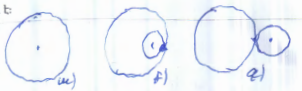
\includegraphics[scale=1]{images_for_internal_reference/id35.png}
%\end{center}
\par Ապա $\R^2 \setminus C$ ենթատարածությունը ունի ա) դեպքում երկու, իսկ բ) և գ) դեպ\-քե\-րում երեքական կապակցվածության բաղադրիչներ (\textbf{որո՞նք են դրանք}):
% 45 +
\end{example}
\begin{theorem}\label{ch14thm8}
\label{15:թեորեմ 8}
Տոպոլոգիական տարածության կապակցվածության բաղադրիչների քանակությունը (ընդհանուր դեպքում որպես բազմության հզորություն) տոպո\-լո\-գի\-ա\-կան ինվարիանտ է։
% 46 +
\par Մասնավորապես դա նշանակում է, որ եթե ինչ-որ տոպոլոգիական տարածու\-թ\-յուն ունի վերջավոր քանակով՝ ճիշտ $n$ հատ կապակցվա\-ծության բաղադրիչ, ապա նրան հոմեոմորֆ ամեն մի տարածություն նույնպես ունի ճիշտ $n$ հատ կապակցվա\-ծության բաղադրիչ։
\end{theorem}
% 47 +
\begin{proof}
Դիցուք $X$-ը և $Y$-ը հոմեոմորֆ տարածություններ են։ Նշանակում է՝ գոյություն ունեն $f:X \rightarrow Y,\ g:Y \rightarrow X$ անընդհատ արտապատկերումներ, որ $f \circ g=\nuynakan_Y$ և $g \circ f=\nuynakan_X$: Նշանակենք $N(X)$-ով և $N(Y)$-ով համապատասխանաբար $X$-ի և $Y$-ի կապակցվածության բաղադրիչների քանակությունները։
% 48 +
\par Այժմ նկատենք, որ $X$-ի ամեն մի կապակցվածության բաղադրիչի կերպարը $f$ անընդհատ արտապատկերման դեպքում ընկած է $Y$-ի որևէ կապակցվածության բաղադրիչի մեջ։ Իրոք, դիցուք $A \subset X,\ B \subset Y$ ենթաբազմությունները կապակց\-վա\-ծության բաղադրիչներ են, ընդ որում $f(A) \cap B \neq \varnothing$։ Ուստի $f(A) \cup B$-ն $Y$-ի կա\-պա\-կցված ենթաբազմություն է համաձայն \hyperref[15:թեորեմ 2]{թեորեմ 2}-ի և \hyperref[15:թեորեմ 3]{թեորեմ 3}-ի։ Կապակց\-վա\-ծու\-թյան բաղադրիչի սահմանումից հետևում է, որ $f(A) \subset B$։ Նշանակում է՝ $N(X)\leq N(Y)$։ Կատարելով նույն դատողությունները $g$ արտապատկերման նկատ\-մամբ՝ ստանում ենք $N(Y)\leq N(X)$, ուստի $N(X)=N(Y)$: 
\end{proof}
% 49 +
\par Որպես հետևանք \hyperref[15:թեորեմ 8]{թեորեմ 8}-ից ստանում ենք, որ \hyperref[15:օրինակ 3]{օրինակ 3}-ում բերված $\R^2 \setminus C$ տարածությունները հոմեոմորֆ չեն միմյանց ա) և բ), կամ ա) և գ) դեպքերում, իսկ բ) և գ) դեպքում $\R^2 \setminus C$ տարածություն\-ների հոմեոմորֆության վերաբերյալ \hyperref[15:թեորեմ 8]{թեորեմ 8}-ը ոչինչ չի տալիս։
% 50 +
\begin{example}\label{ch14ex4}
Դիտարկենք հայոց այբուբենի \inlinegraphics{\import{tikz/Letter A/}{a_capital.tex}} և \inlinegraphics{\import{tikz/Letter A/}{a.tex}} տառերը (գծապատ\-կեր\-նե\-րը) որպես $(\R^2, \textrm{սովոր.})$ տարածության ենթատարածություններ։ Հարց․ արդյոք հոմեո\-մո՞րֆ են դրանք միմյանց։ 
\end{example}
\label{15:օրինակ 3}
% 51 +
\par Նկատենք, որ եթե հնարավոր է երկու գծապատկերներից մեկը անընդհատ ձևա\-փոխելով, առանց կտրատելու և առանց ինքնահատումների համընկեցնել մյուսի հետ, ապա դրանք հոմեոմորֆ են։ Տվյալ դեպքում հարցի պատասխանը դրական է, և օրինակ հոմեոմորֆիզմ կարելի է կառուցել հետևյալ հաջորդականությամբ՝
% 52
\import{tikz/Letter A/}{Atoa.tex}
\par Այժմ քննարկենք նույն հարցը \inlinegraphicslower{\import{tikz/Letter A/}{NA.tex}} և
\inlinegraphics{\import{tikz/Letter A/}{a.tex}}
գծապատկերների համար։ Այս դեպ\-քում բոլոր փորձերը նախորդի նմանությամբ մի պատկերից ստանալ մյուսը դատա\-պարտ\-ված են ձախողման։ Պատճառը այդ պատկերների կառուցվածքային էական տար\-բե\-րութ\-յան մեջ է․ եթե մենք \inlinegraphics{\import{tikz/Letter A/}{a.tex}} պատկերից հեռացնենք մի որևէ կետ, ապա ստացված պատկերը կարող է լինել ոչ կապակցված տարածություն, որի կապակց\-վա\-ծության բաղադրիչների քանակությունը կարող է լինել ամենաշատը երեք։ Իսկ եթե նման գործողություն կատարենք \inlinegraphicslower{\import{tikz/Letter A/}{NA.tex}} պատկերի հետ, ապա կախված հեռացվող կետից կարող է ստացվել տարածություն, որն ունի կապակցվածության չորս բա\-ղադրիչ։ Այժմ, օգտագործելով այս հանգամանքը՝ ապացուցենք, որ այս պատկեր\-ները հոմեմորֆ չեն միմյանց։
% 53
\par Իրոք, ենթադրենք գոյություն ունի $h:$ \inlinegraphicslower{\import{tikz/Letter A/}{NA.tex}}  $\rightarrow$ \inlinegraphics{\import{tikz/Letter A/}{a.tex}} հոմեոմորֆիզմ։ Հեռացնենք \inlinegraphicslower{\import{tikz/Letter A/}{Awitha.tex}} պատկերից $a$ կետը, իսկ \inlinegraphics{\import{tikz/Letter A/}{a.tex}} պատկերից $h(a)$ կետը։ 

\par Ստացված $\widebar{h}:$ \inlinegraphicslower{\import{tikz/Letter A/}{NA.tex}} $\setminus \, \{a\} \rightarrow$ \inlinegraphics{\import{tikz/Letter A/}{a.tex}} $\setminus \  \{h(a)\}$ արտապատկերումը նորից հոմեոմոր\-ֆիզմ է (ինչո՞ւ)։ Բայց \inlinegraphicslower{\import{tikz/Letter A/}{NA.tex}} $\setminus\, \{a\}$ տարածությունն ունի կապակցվածության 4 բաղա\-դրիչ, մինչդեռ \inlinegraphics{\import{tikz/Letter A/}{a.tex}} $\setminus\ \{h(a)\}$ տարածության համար դրանց քանակությունը փոքր է 4-ից (հակասություն \hyperref[15:թեորեմ 8]{թեորեմ 8}-ի հետ)։
% 54
\par Անդրադառնալով տարածությունների միջև հոմեոմորֆիզմ կառուցելու խնդրին՝ կատարենք կարևոր դիտողություն։ Եթե մի տարածություն (օրինակ՝ գծապատկեր) հնարավոր չէ առանց կտրատումների և ինքնահատումների համընկեցնել մյուսի հետ, դա դեռ չի նշանակում, որ այդ տարածությունները հոմեոմորֆ չեն։
% 55
\par Օրինակ՝ $\R^3$ տարածությունում հնարավոր չէ առանց ինքնահատումների $x^2+y^2=r^2,\ z=0$ շրջանագիծը անընդհատ ձևափոխումներով համընկեցնել այսպես կոչված «երեքնուկաձև» օվալի հետ։ Մինչդեռ դրանք հոմեոմորֆ են միմյանց։
% 56

% բերված է թեմա 11-ի խնդիրներից
\begin{center}
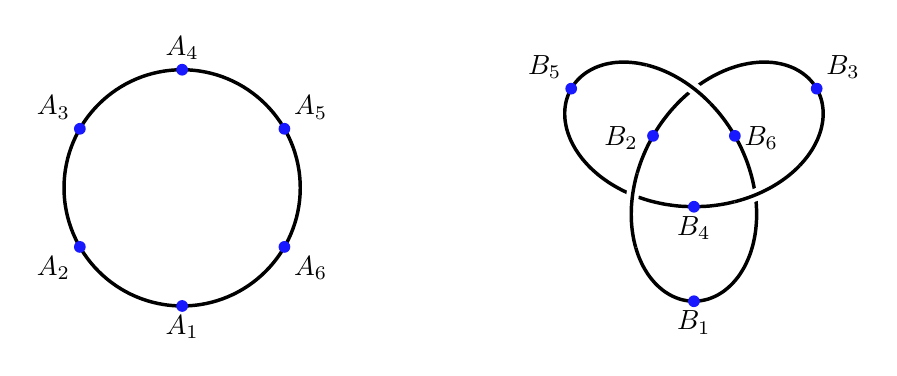
\begin{tikzpicture}[
    scale=1.0,
    every node/.style={text=black},
    dot/.style={circle, fill=blue!90, inner sep=1.5pt}
]

    % ==========================
    % LEFT FIGURE: The Circle
    % ==========================
    \begin{scope}[xshift=0cm]
        \draw[line width=1.25pt, black] (0,0) circle (1.5cm);

        % Brace the position values to prevent 'unknown key' error
        \foreach \i/\angle/\pos in {
            1/270/below, 
            2/210/{below left}, 
            3/150/{above left}, 
            4/90/above, 
            5/30/{above right}, 
            6/-30/{below right}} 
        {
            \node[dot] (A\i) at (\angle:1.5cm) {};
            \node[\pos] at (A\i) {$A_{\i}$};
        }
    \end{scope}


    % ==========================
    % RIGHT FIGURE: The Trefoil Knot
    % ==========================
    \begin{scope}[xshift=6.5cm, scale=0.6, yshift=0.6cm] 
        
        % NOTE: Removed the negative sign from Y coordinate to flip the shape
        % vertically so it points DOWN (matching your B1 at bottom sketch).
        
        % 1. Draw the FULL knot (Background)
        \draw[line width=1.25pt, color=black] plot[domain=0:360, samples=100, smooth] 
            ({-(sin(\x) + 2*sin(2*\x))}, {(cos(\x) - 2*cos(2*\x))});

        % 2. Draw "Over" segments (Halo Effect)
        
        % Crossing 1 (Bottom Right area in this orientation)
        \draw[line width=4.5pt, color=white] plot[domain=90:110, samples=20, smooth] 
             ({-(sin(\x) + 2*sin(2*\x))}, {(cos(\x) - 2*cos(2*\x))});
        \draw[line width=1.25pt, color=black] plot[domain=90:110, samples=20, smooth] 
             ({-(sin(\x) + 2*sin(2*\x))}, {(cos(\x) - 2*cos(2*\x))});

        % Crossing 2 (Top Center area)
        \draw[line width=4.5pt, color=white] plot[domain=210:230, samples=20, smooth] 
             ({-(sin(\x) + 2*sin(2*\x))}, {(cos(\x) - 2*cos(2*\x))});
        \draw[line width=1.25pt, color=black] plot[domain=210:230, samples=20, smooth] 
             ({-(sin(\x) + 2*sin(2*\x))}, {(cos(\x) - 2*cos(2*\x))});

        % Crossing 3 (Bottom Left area)
        \draw[line width=4.5pt, color=white] plot[domain=330:350, samples=20, smooth] 
             ({-(sin(\x) + 2*sin(2*\x))}, {(cos(\x) - 2*cos(2*\x))});
        \draw[line width=1.25pt, color=black] plot[domain=330:350, samples=20, smooth] 
             ({-(sin(\x) + 2*sin(2*\x))}, {(cos(\x) - 2*cos(2*\x))});

        % 3. Place Labels B1...B6
        % Adjusted angles for the flipped (Point Down) orientation
        \foreach \i/\t/\pos in {
            1/180/below,        
            2/240/{below left, yshift=7pt, xshift=-2pt}, 
            3/300/{above right, yshift=0pt}, 
            4/0/below,          
            5/60/{above left, yshift=0pt}, 
            6/120/{below right, yshift=7pt}} 
        {
            % Calculate coordinate
            \pgfmathsetmacro{\px}{-(sin(\t) + 2*sin(2*\t))}
            \pgfmathsetmacro{\py}{(cos(\t) - 2*cos(2*\t))} % Removed minus here too
            
            \node[dot] (B\i) at (\px,\py) {};
            \expandafter\node\expandafter[\pos] at (B\i) {$B_{\i}$};
        }
        
    \end{scope}

\end{tikzpicture}
\end{center}


% \import{tikz/uniform/}{37.tex}
%\begin{center}
%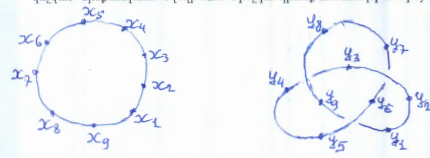
\includegraphics[scale=1]{images_for_internal_reference/id37.png}
%\end{center}
\par Իրոք, վերցնելով շրջանագծի վրա $A_1, A_2, \dots, A_6$ կետերը, իսկ օվալի վրա $B_1$, $B_2, \dots, B_6$ կետերը՝ մենք կարող ենք նախ կառուցել հոմեոմորֆիզմներ այդ պատ\-կեր\-ների համա\-պա\-տաս\-խան աղեղների միջև՝ ${h_1:A_1 A_2 \rightarrow B_1 B_2,\ h_2:A_2 A_3 \rightarrow B_2 B_3}$, $\dots$, $h_5:A_5 A_6 \rightarrow B_5 B_6,\ h_6:A_6 A_1 \rightarrow B_6 B_1$։ Այնուհետև հաջորդաբար «սոսնձելով» այդ արտապատկերումներից յուրաքանչյուրն իր հաջորդի հետ (թեմա 11-ում \hyperref[ch11thm3]{թեո\-րեմ 3}-ի իմաստով)՝ կստանանք որոնելի $h$ հոմեոմորֆիզմ։

\bigskip
\bigskip
\subsubsection*{Խնդիրներ և հարցեր թեմա 14-ի վերաբերյալ}

\begin{enumerate}[label=\thesection.\arabic*.]

% 15.1
\item Ճի՞շտ է պնդումը․ կապակցված տարածության ցանկացած ենթաբազ\-մու\-թյուն կապակցված է։

% 15.2
\item Ապացուցեք․ կապակցված $X$ տարածության ցանկացած $\faktor{X}{R}$ ֆակտոր-տարա\-ծություն կապակցված է։

% 15.3
\item Ապացուցեք․ $(\R, \text{սովոր.})$ տարածության ռացիոնալ կետերի ամեն մի ենթա\-բազ\-մություն կապակցված չէ։

% 15.4
\item Ունենք $f: X \to Y$ անընդհատ արտապատկերում։ Ճի՞շտ է պնդումը․ $Y$-ում կա\-պա\-կցված ամեն մի $B$ ենթաբազմության $f^{-1}(B)$ նախակերպարը կապա\-կց\-ված է $X$-ում։

% 15.5
\item Ապացուցեք․ $\R^n$ էվկլիդեսյան տարածության ամեն մի ուռուցիկ ենթա\-բազ\-մություն կապակցված ենթատարածություն է:
\begin{hint}
Սևեռելով $X \subset \R^n$ ուռուցիկ ենթաբազմության որևէ $x_0$ կետ՝ դի\-տար\-կեք $x_0$ սկզբնակետով բոլոր հատվածները, որոնք ընկած են $X$-ում:
\end{hint}

% 15.6
\item $\R^3$ էվկլիդեսյան տարածության հետևյալ երեք՝
\[
\big\{(x,y,z); \; x^2+y^2-z^2=\delta\big\}, 
\qquad \text{որտեղ } \delta=-1, 0, 1
\] 
մակերևույթներից որո՞նք են կապակցված (պատասխանը հիմնավորե՛ք):

% 15.7
\item Ճի՞շտ է արդյոք պնդումը․ $(\R, \mapsto)$ տարածության հետևյալ ենթա\-բազ\-մու\-թյուն\-ներից՝ ա) $\{0,1\}$, բ) $[0,1)$, գ) $[0,1]$, դ) $(0,0)$, ե) $(0,1]$, ոչ մեկը կապակցված չէ:

% 15.8
\item Ապացուցեք․ $\R^2$ էվկլիդեսյան հարթության այն բոլոր կետերի $A$ ենթա\-բազ\-մու\-թյունը, որոնց կոորդինատներից գոնե մեկը ռացիոնալ թիվ է, կապակցված ենթա\-բազմություն է:
\begin{hint}
Հիմնավորեք, որ $A$-ի ցանկացած երկու կետեր կարող են միացվել իրար երկու կամ երեք հատվածներից կազմված բեկյալով, որն ամբողջությամբ ընկած է $A$-ի մեջ:
\end{hint}

% 15.9
\item Ճի՞շտ է արդյոք, որ $\R^2$ հարթության այն բոլոր կետերի $B$ ենթաբազմությունը, որոնց կոորդինատներից միայն մեկն է ռացիոնալ թիվ, կապակցված ենթա\-բազ\-մություն է:
\begin{hint}
Ըստ պայմանի՝ $B$-ն չունի ընդհանուր կետ $y=x$ ուղղի հետ։ Ուստի $B$-ն ներկայացվում է որպես երկու ենթաբազմությունների միավորում, որոնցից մեկը ընկած է այդ ուղղից վերև, իսկ մյուսը՝ ներքև:
\end{hint}

% 15.10
\item Ապացուցեք․ $\R$ թվային ուղղի որևէ $[a,b]$ ենթատարածություն հոմեոմորֆ չէ $\R^2$ հարթության որևէ $[c,d] \times [e,f]$ ենթատարածության:

% 15.11
\item Ապացուցեք․ $X$ տոպոլոգիական տարածությունը կապակցված է այն և միայն այն դեպքում, երբ ցանկացած $f: X \to Y$ անընդհատ արտապատկերում, որ\-տեղ $Y$-ը մեկից ավելի կետեր պարունակող դիսկրետ տարածություն է, հաս\-տա\-տուն արտապատկերում է:

% 15.12
\item Ապացուցեք․ $(X, \tau)$ տոպոլոգիական տարածությունը կապակցված չէ այն և մի\-այն այն դեպքում, երբ գոյություն ունի $f: (X, \tau) \to (Y, \text{դիսկր.})$ անընդհատ սյուրյեկտիվ արտապատկերում, որտեղ $Y$-ը երկկետանոց բազմություն է:

% 15.13
\item Ապացուցեք․ եթե $A$-ն $X$ տարածության կապակցված ենթատարածություն է և $A \subset Y \subset \overline{A}$, ապա $Y$-ը $X$-ի կապակցված ենթատարածություն է:

\end{enumerate}


\end{document}